\documentclass[10pt, a4paper]{article}
\usepackage[brazil]{babel}
\usepackage[utf8]{inputenc}
\usepackage[T1]{fontenc}
\usepackage{url}
\usepackage{lscape}
\usepackage{tabularx}
\usepackage{longtable}
\usepackage{setspace}
\usepackage[pdftex]{graphicx}
\usepackage[usenames,svgnames,dvipsnames]{xcolor}
\graphicspath{{./imagens/}}
\usepackage{color}
\usepackage{physics}
\usepackage{indentfirst}
\usepackage{float}

\usepackage[demo]{graphicx}
\usepackage{caption}
\usepackage{subcaption}

\setlength{\parskip}{2mm}
\usepackage[a4paper,top=2.0cm,bottom=2.0cm,left=2.0cm,right=2.0cm]{geometry} 
\usepackage[round,sort,nonamebreak]{natbib}  
\bibpunct{(}{)}{;}{a}{,}{,}

\usepackage{fancyhdr}
\pagestyle{fancy}

\usepackage[font=small,format=plain,labelfont=bf,up,textfont=it,up]{caption}
\usepackage[pdftex,plainpages=false,pdfpagelabels,
	linktocpage,
	colorlinks=true,
	citecolor=DarkGreen,
	linkcolor=NavyBlue,
	urlcolor=DarkRed,
	filecolor=green,
	bookmarksopen=true,
	pdfauthor={Nome do autor do documento},
	pdfsubject={subject1, subject2, ...},
	pdfkeywords={keyword1, keyword2, ...}
]{hyperref}

\singlespacing  


% ------------------------------------------------------------------ %
\begin{document}
\lhead{  Laboratório avançado de ciência de dados  }
\rhead{USP}

\title{\textbf{   Análise descritiva  \\
                Transparência em Tempos de Pandêmia
                }\\[2em] }

\author{ Gabriel Martins Trettel - N. USP 11389471  \\
         George Othon Silva Santos - N. USP 10349978 \\
         Tiago Lubiana Alves - N. USP 8945857 \\
         Wesley Seidel Carvalho - N. USP 6544342 \\
        }
\date{  São Paulo, 08 de Setembro de 2020  }
% Santo André, 21 de Setembro de 2018
\maketitle

\section{ Descrição inicial da proposta }

Neste trabalho descrevemos o entendimento inicial do problema apresentado pelo cliente Open Knowledge Brasil (OKB) tendo como contato o sr. Mário. Também descrevemos os dados que nos foram apresentados e a forma com a qual foram obtidas pelo cliente. O trabalho diz respeito à análise de dados textuais extraídos de diversos diários oficiais.

Uma primeira reunião com o cliente foi realizada no dia 04/09/2020, na qual estiveram presentes o sr. Mário Queiroz e Ariane representando a OKB e a equipe de desenvolvimento deste trabalho. Após conversa com os representantes da OKB, começamos a definir os objetivos do projeto.

Devido a riqueza dos dados e a natureza múltipla dos interesses do cliente, pautamos um objetivo inicial para orientar a exploração dos dados: Um dos desejos citados pela equipe da OKB é que em algum momento, os interessados em informações dos Diários Oficiais  consigam identificar compras suspeitas durante a pandemia. Neste caso, a tarefa consistirá tanto em identificar compras e contratações feitas em determinado período quanto em organizar tais informações e possibilidades de integração com bases de dados sugeridas pelo cliente, tais como a base de sócios de empresas brasileiras e a base de dados de doações de campanha do Tribunal Superior Eleitoral.

Tal tarefa implica, à priori, extração de informações dos diários tais como: valores envolvidos em transações; partes envolvidas nas transações; data das transações. A partir disso, então, será possível pensar em estratégias para identificar situações que possam ser consideradas suspeitas, a exemplo de donos de empresas envolvidas tanto com financiamento de campanhas nas eleições de 2020 como em transações comerciais relatadas em diário oficial.

Algumas palavras sobre a exploração dos dados piloto dos Diários Oficiais: Os dados foram fornecidos em diversas pastas, com categorias distintas. Os arquivos estão presentes em formato txt, com diversos arquivos por pasta. Neste documento realizamos algumas análises iniciais sobre esta massa de dados além da discussão de algumas possibilidades de implementação que nos auxilie em definir objetivos mais claros e auxilie o cliente no vislumbre de um produto viável.

\subsection{Descrição da organização dos dados}

A descrição dos dados, nos fornecida pelo Mario Sérgio, nosso ponto de contato da \textit{Open Knowledge Foundation}, é a seguinte:

Foram coletados arquivos em PDF de 306 municípios brasileiros, listados em um \href{https://github.com/okfn-brasil/querido-diario/tree/main/processing/data_collection/gazette/spiders}{repositório} no \textit{GitHub} da organização.
O intervalo de publicação dos diários é do dia 01 de fevereiro de 2020 até o dia 15 de junho de 2020. Os arquivos foram convertidos de PDF para txt e, então, uma busca por palavras-chave foi exexutada para tentar separa-los por assunto. As palavras-chaves utilizadas foram:

\begin{itemize}
    \item Emergencial
    \item Estado de Emergência de Saúde Pública
    \item Dispensa de licitação
    \item Equipamentos de Proteção Individual
    \item EPI
    \item Ventiladores pulmonares
    \item Ventilador pulmonar
    \item Demanda Emergencial Covid-19
    \item Teste rápido
    \item RT-PCR
    \item Hospital de Campanha
\end{itemize}

Pela natureza do que foi nos dado, não temos de maneira direta a informação dos municípios do qual cada diário foi obtido, nem suas respectivas datas de publicação. Iremos tentar obter essa informação para as etapas seguintes do processo, após interagir com a equipe responsável pelo \textit{scraping} das páginas dos municípios. 


\section{Descrevendo os arquivos apresentados} 


Tendo em vista que os dados foram provenientes de buscas por palavras-chave, decidimos ver o número de arquivos para cada busca, visto na tabela \ref{tab:quantidade_arquivo_p_pasta}:

\begin{table}[H]
    \centering
    \centering
    \begin{tabular}{|l|c|c|}
    \hline
        Termo de busca                            & Qnt & (MB) \\ \hline
        Demanda Emergencial Covid-19              & 228 & 109M \\
        \_Dispensa de licitação\_                 & 800 & 290M \\
        emergencial                               & 440 & 198M \\
        EPI                                       & 223 & 140M \\
        \_Equipamentos de Proteção Individual\_   & 207 & 116M \\
        \_estado de Emergência de Saúde Pública\_ & 36 & 20M \\
        \_Hospital de Campanha\_                  & 52 & 12M \\
        RT-PCR                                    & 26 & 16M \\
        \_teste rápido\_                          & 56 & 35M \\
        \_ventiladores pulmonares\_               & 10 & 6,6M \\
        \_ventilador pulmonar\_                   & 18 & 12M \\ \hline
        Total                                     & 2108 & 950MB \\ \hline

    \end{tabular}
    \caption{Quantidade de arquivos para cada diretório que representa um termo de busca}
    \label{tab:quantidade_arquivo_p_pasta}
\end{table}

Apesar do número de arquivos variar entre as buscas, a proximidade semântica dos termos buscados nos levou à hipótese que poderia haver redundância no conjunto de dados. Ou seja, o mesmo arquivo poderia ter sido recuperado independentemente em duas ou mais buscas. 
 
 % A partir daqui, é texto novo
De fato, esta hipótese está verificada, já que ao analisarmos o conteúdo de todos os arquivos, foi visto que apenas 1011 deles são de fato únicos e, cada um deles, poderia estar presente em pelo menos 1 e até 11 das categorias distintas. Então contamos quantos diretórios cada arquivo está presente. Na tabela \ref{tab:quantidade_arquivo_p_pasta}, a primeira coluna representa a quantidade de diretórios que cada arquivo está e a segunda coluna a quantidade de arquivos que tem essa propriedade

\begin{table}[H]
    \centering
    \begin{tabular}{c|c}
        Diretórios com arquivos duplicados & Quantidade de arquivos \\ \hline
        1 &  474 \\
        2 &  242 \\
        3 &  156 \\
        4 &  65  \\
        5 &  45  \\
        6 &  19  \\
        7 &  10  \\
        \hline
        total & 1011 \\
    \end{tabular}
    \caption{Quantidade de diretórios que um mesmo arquivo pode pertencer pela quantidade de arquivos.}
    \label{tab:my_label}
\end{table}

\subsection{Formatação dos dados}

Cada arquivo é uma representação em texto de um documento que originalmente estava em PDF, por conta disso, a formatação dos diários acaba sendo embutida também nos \textit{txt's}. Com isso, cada arquivo que temos em mãos possui uma formatação distinta entre cada um deles e até entre as páginas do mesmo. Alguns possuem o \textit{layout} disposto em colunas, sendo observados de 2 até 4, outros possuem colunas em algumas páginas e outras apenas um corpo centralizado. Existem diários que possuem tabelas dentro do documento.

Durante o processo de conversão dos PDF's para o txt, algumas informações se perderam tais como a quebra de página. O documento de texto é contínuo durante todo seu comprimento, por isso, precisamos recorrer a heurísticas para determinar onde uma página termina e outra começa. O processo descoberto por nós se deu ao abrir os documentos num editor de texto chamado Vim, que mostra um caractere cinza-claro\ref{fig:quebra_de_pagina} justamente na primeira linha de cada página. Este caractere pode ser procurado utilizando expressão regular ou alguma outra ferramenta de busca em textos pelo código  \texttt{\textbackslash 014.}

\begin{figure}[H]
    \centering
    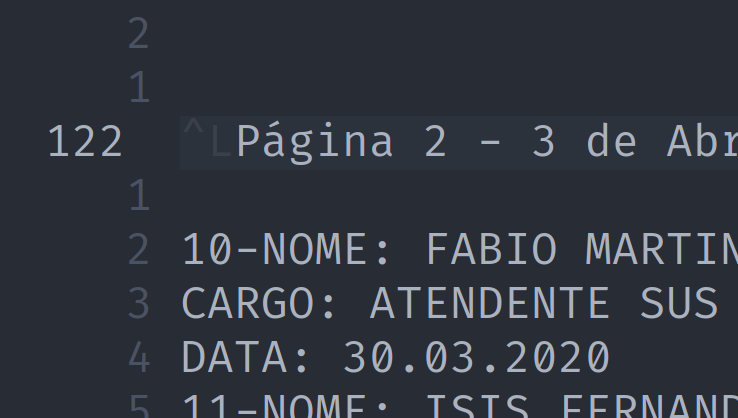
\includegraphics[scale=0.4]{images/prints/quebra_pagina.png}
    \caption{O primeiro caractere da linha 122,  \texttt{\textasciicircum L}, aparece em toda primeira linha das segunda página em diante}
    \label{fig:quebra_de_pagina}
\end{figure}

Outro problema relacionado com a conversão dos formatos é a manutenção do layout original do PDF, os documentos costumam ter sessões com múltiplas colunas ou tabelas em seu conteúdo. Nada disso sendo padronizado durante a extensão do documento. Como exemplo, podemos verificar o conteúdo do arquivo \texttt{122.txt}, que possui algumas páginas com 2 colunas \ref{fig:duas_colunas}, mas também possui tabelas \ref{fig:tabela} e uma combinação de texto com tabela \ref{fig:tabela}.

\begin{figure}[H]
    \centering
    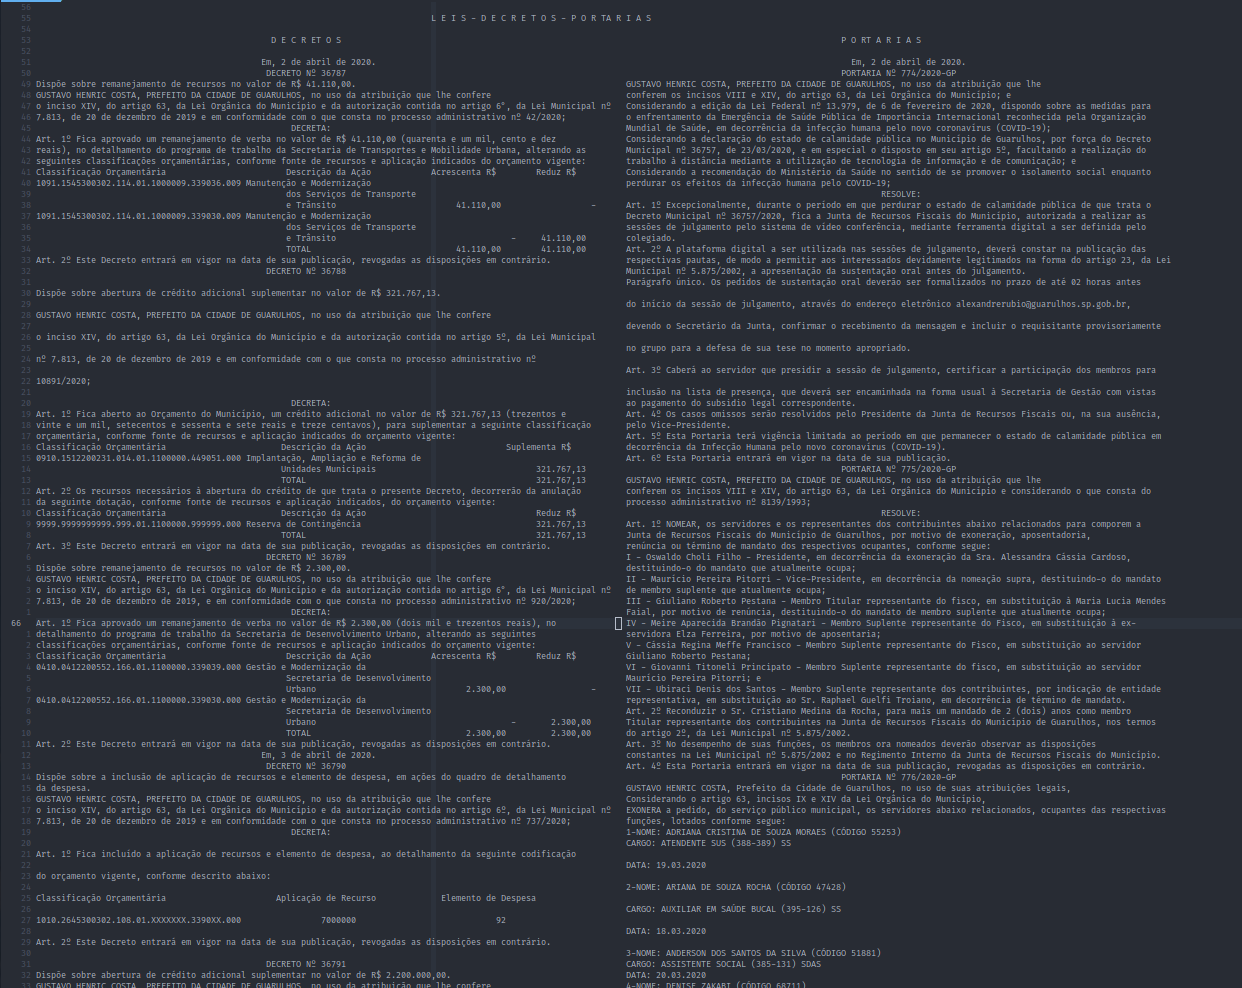
\includegraphics[scale=0.2]{images/prints/colunas.png}
    \caption{Exemplo de uma página que possui duas colunas}
    \label{fig:duas_colunas}
\end{figure}

\begin{figure}[H]
    \hfill
    \subfloat[\centering Apenas tabela ]{{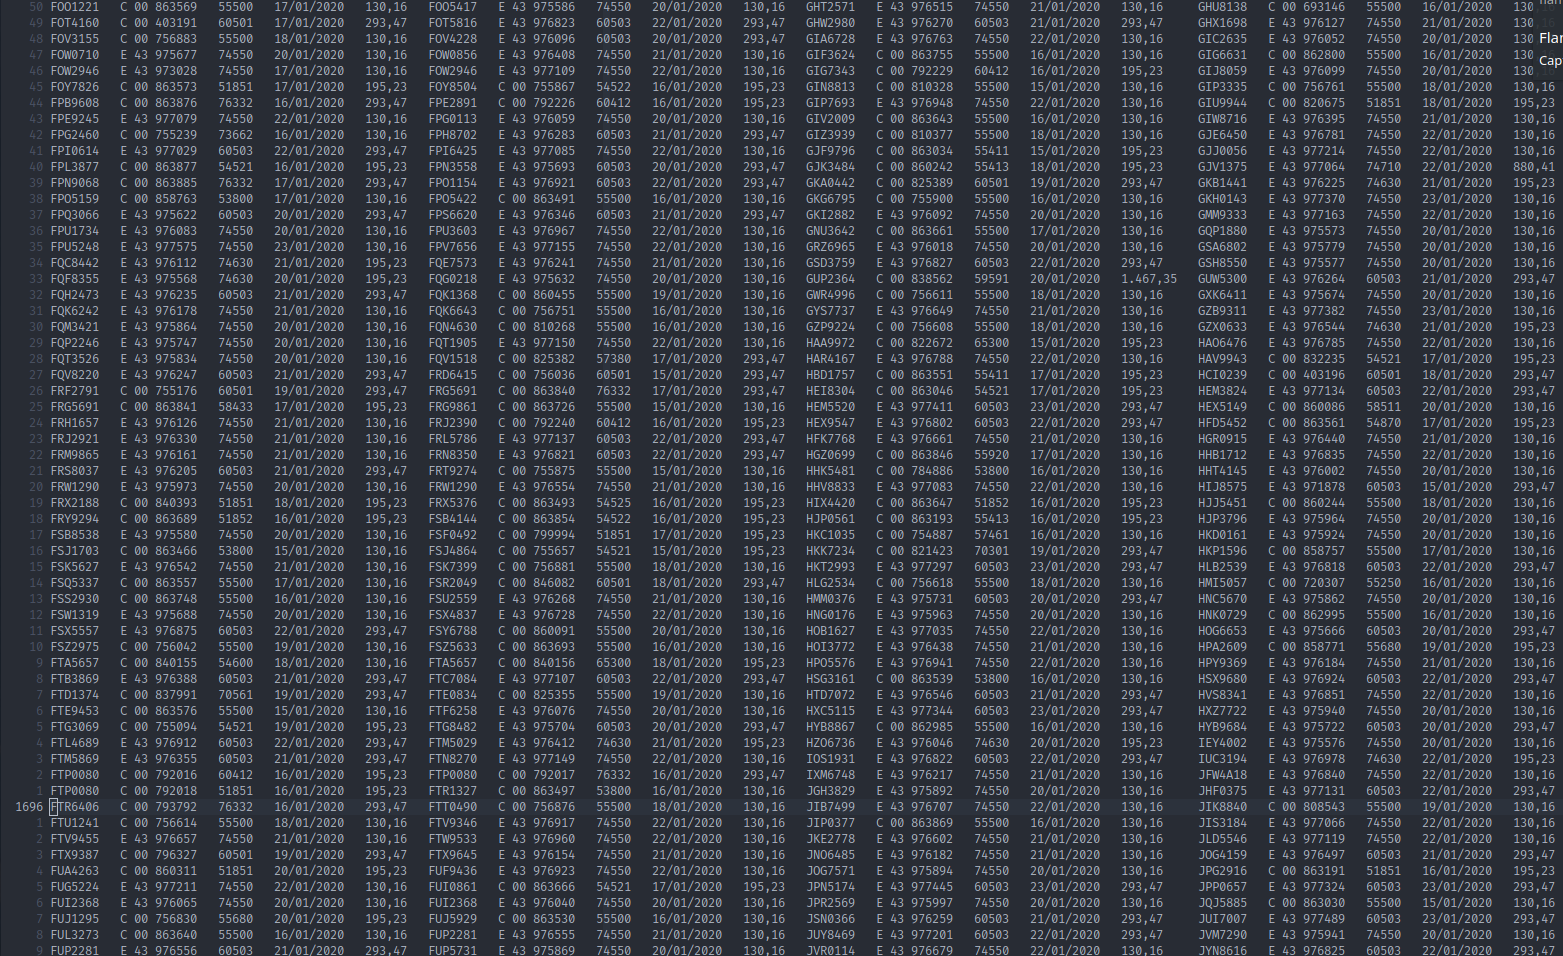
\includegraphics[width=.45\linewidth]{images/prints/tabelas} }}%
    \hfill
    \subfloat[\centering Tabela com texto ]{{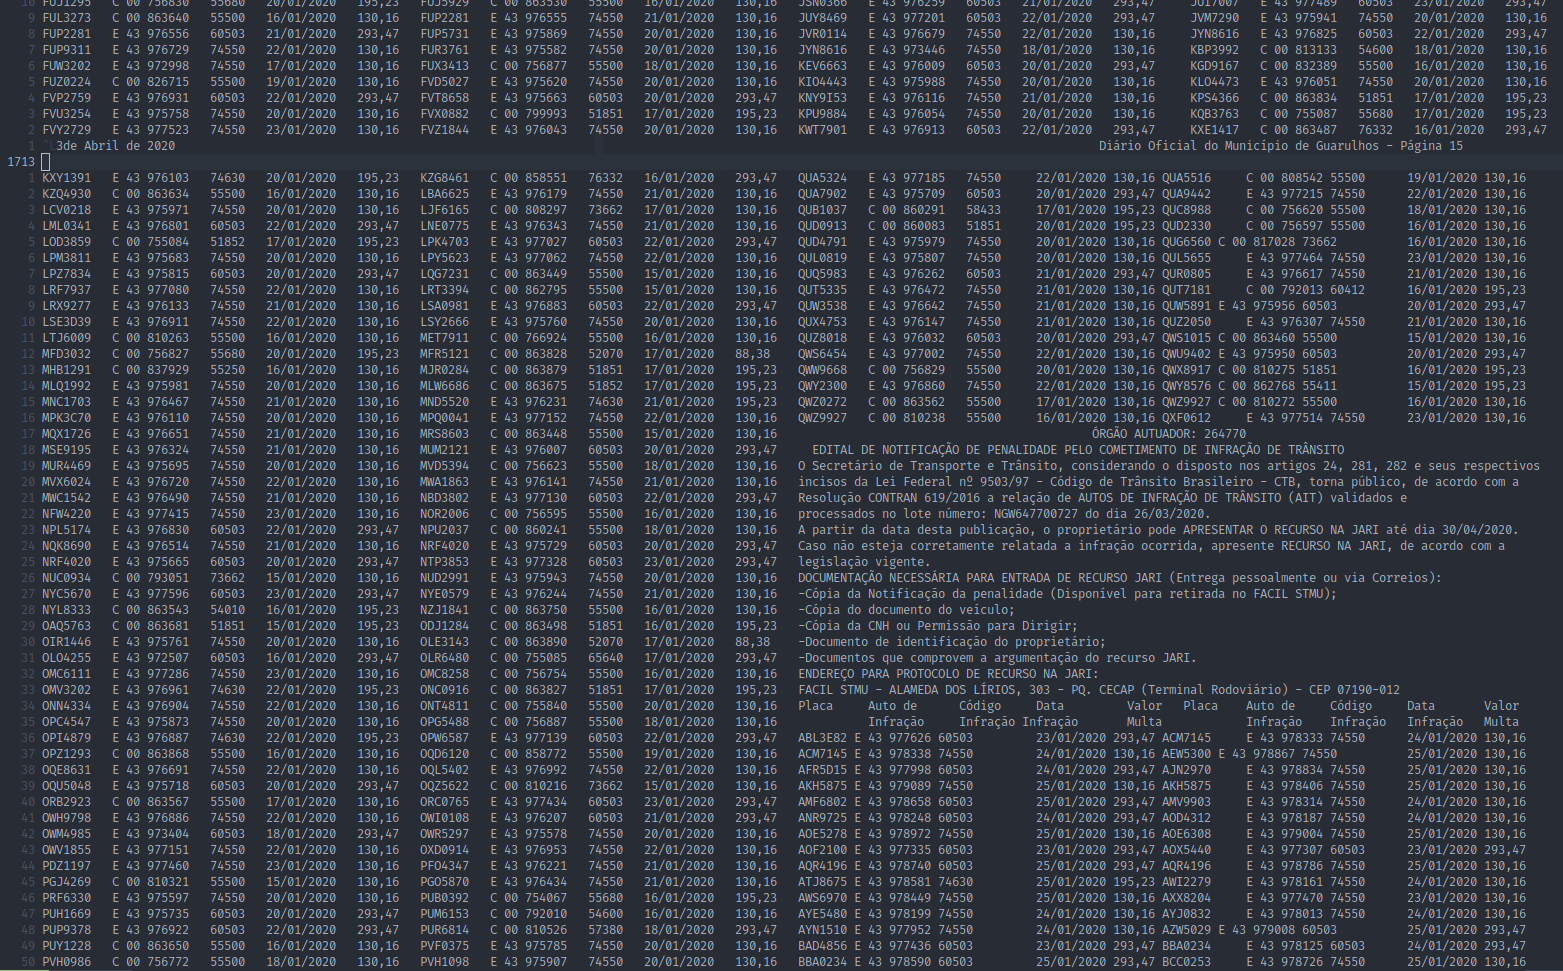
\includegraphics[width=.45\linewidth]{images/prints/texto_com_tabelas} }}%
    \hfill

    \caption{Formas que tabelas podem aparecer no texto}
    \label{fig:tabela}
\end{figure}


Entender esse tipo de detalhe de formatação é importante para nosso objetivo, pois, muitas das análises de texto acabam precisando recuperar informações relacionadas ao contexto das palavras, i.e, outras palavras que estão ao seu redor. Para recuperar termos que estão na vizinhança, temos que transformar as colunas (quando houverem) para um texto sequencial. Apenas com o texto separado a coleta de \textit{n-gramas} se torna possível. Portanto, desenvolver um algoritmo ou heurística que consiga separar as colunas do texto e dispô-las de forma sequencial é imprescindível antes de qualquer análise mais sofisticada. Como não temos conhecimento de nada já pronto que faça o trabalho, decidimos que uma solução autoral seria desenvolvida, mas, para isso, precisamos entender com mais detalhes como este fenômeno ocorre.

Durante uma análise visual dos textos, percebemos que o espaço entre palavras da mesma coluna era sempre de uma unidade e que na grande maioria das linhas as colunas tinham um espaçamento mínimo de dois espaços. Por conta disso a forma que desenvolvemos para calcular a quantidade de colunas (e seu espaçamento) se dá justamente nesta quase padronização. A análise que decorre do seguinte procedimento: para cada arquivo, separá-lo em páginas (usando o \texttt{\textasciicircum L} como delimitador) e depois contar, por página, quantas linhas possuem uma sequência de dois ou mais espaços contíguos. Se a linha possui duas sequencias de espaços, então ela possui três colunas. Da mesma forma, se nenhuma sequência for retornada é porque o texto está em apenas uma coluna. Depois de executar este cálculo para todas as linhas da página, calculamos a média aritmética e resultado é a \emph{média de colunas por página por documento}. O espaçamento entre as colunas é similar; calculamos o comprimento das sequências de espaços e depois vemos a média de espaços, também por página. Chamamos isto de \emph{espaçamento médio entre colunas por página por documento}.

O resultado deste método nos retorna, para cada texto, duas listas de números reais. Cada posição dessa lista representa uma das páginas e o valor a média da quantidade de colunas ou do espaçamento entre as colunas. Com essas listas, fizemos dois tipos agrupamentos diferentes: um contando todos os 1011 arquivos distintos como um único corpo, e outro separando pelas categorias de busca. 


Na figura \ref{fig:qtd_colunas} podemos observar duas sub-figuras; a \emph{(a)} representa a quantidade média de colunas considerando todos os documentos e a \emph{(b)} para cada termo de busca. Podemos observar que existem picos perto dos números 1 e 2, indicando que essas são as maiores ocorrências, e, no \textit{boxplot} acima, temos o valor confirmado, com a mediana perto de 1.5. Precisamos levar em conta, portanto, que a maioria das páginas tem 1 ou 2 colunas e poucas tem muito mais do que isso. O maior valor observado foram 13 colunas numa página que continha uma tabela. Agrupando pelos termos de busca observamos uma consistência entre os valores, indicando que não existe quase nenhuma correlação entre a quantidade de colunas e o termo de busca. No caso de \emph{ventiladores pulmonares} e \emph{ventilador pulmonar} observa-se um comportamento um pouco diferente, mas isso se deve pelo desbalanço dos dados, já que segundo a tabela \ref{tab:quantidade_arquivo_p_pasta}, estes são os termos com menos resultados.

\begin{figure}[H]
    \centering
    \hfill
    
    \subfloat[\centering Quantidade média de colunas para todos os documentos ]{{\includegraphics[width=\linewidth]{images/figuras/Quantidade média de colunas por documento.pdf} }}%
    \hfill
    
    \subfloat[\centering Quantidade de colunas para cada categoria de busca ]{{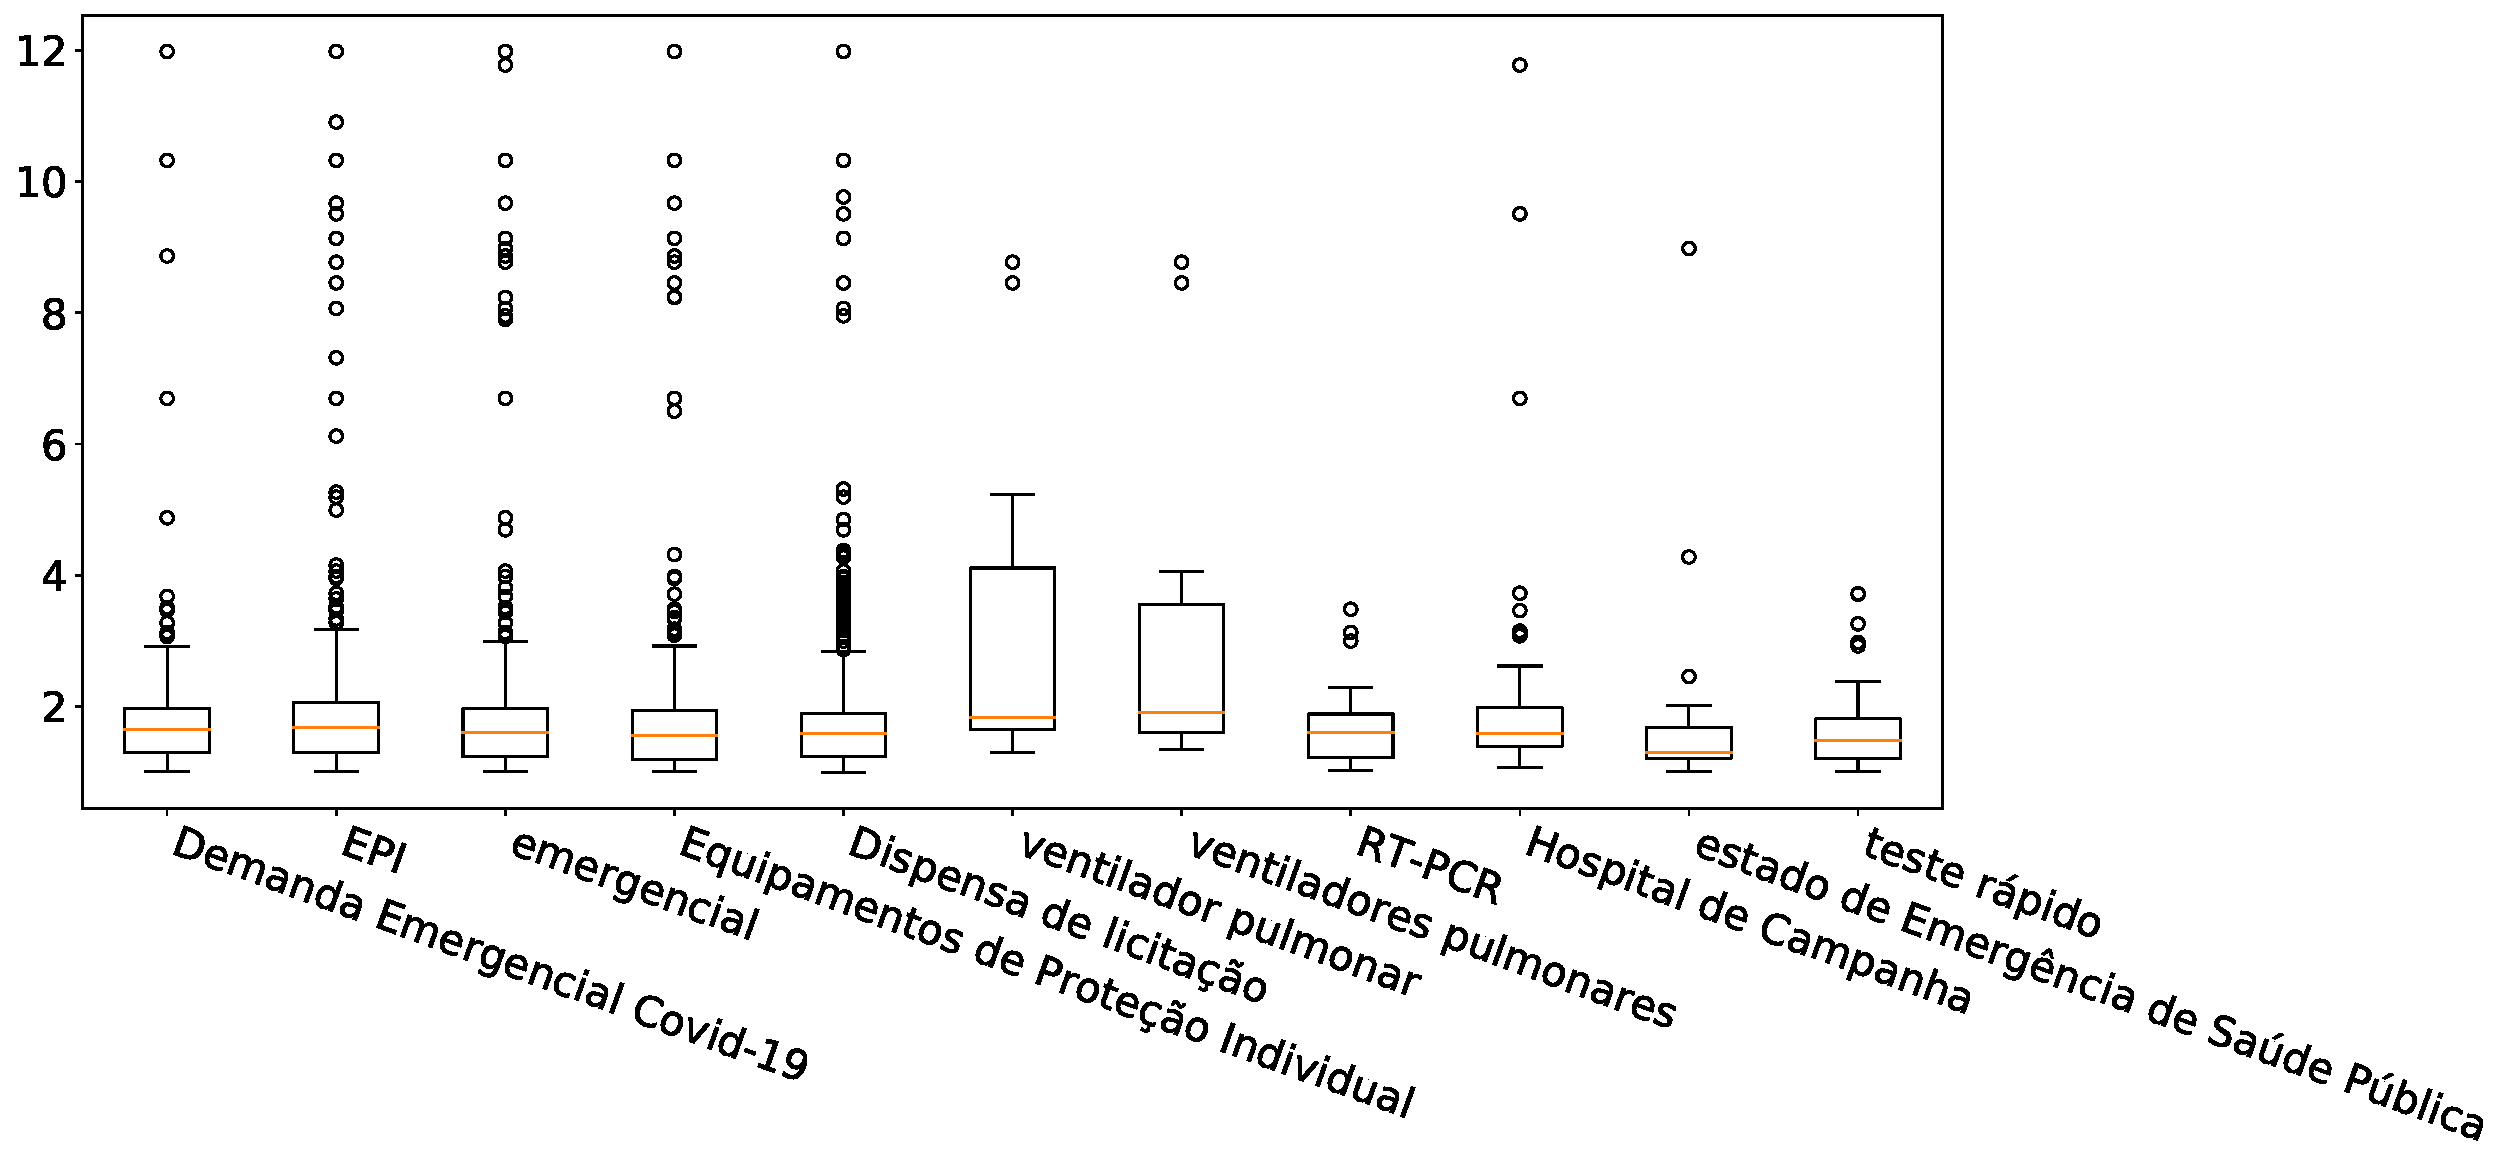
\includegraphics[width=\linewidth]{images/figuras/Quantidade de colunas por cada categoria de busca.pdf} }}%
    \hfill

    \caption{Análise da quantidade de colunas}
    \label{fig:qtd_colunas}
\end{figure}


Observando pelo prisma do espaçamento entre as colunas, na figura \ref{fig:spac_colunas}, existem dois picos bem claros por volta de 2,5 espaços e de 11 espaços, sendo o último o mais frequente. Este resultado é consistente com o da quantidade de colunas, já que nele vemos que existe, principalmente, dois casos, um que temos algo em torno de 1 a 3 espaços (provavelmente nas tabelas) e outro com 10 espaços (provavelmente nas colunas que possuem texto). Não foi observado na figura da quantidade de colunas \ref{fig:qtd_colunas} os dois picos, pois as tabelas variam muito na quantidade de colunas, mas não no espaçamento entre elas.


\begin{figure}[H]
    \centering
    \hfill
    
     \subfloat[\centering  Espaçamento entre as colunas para  todos os documentos ]{{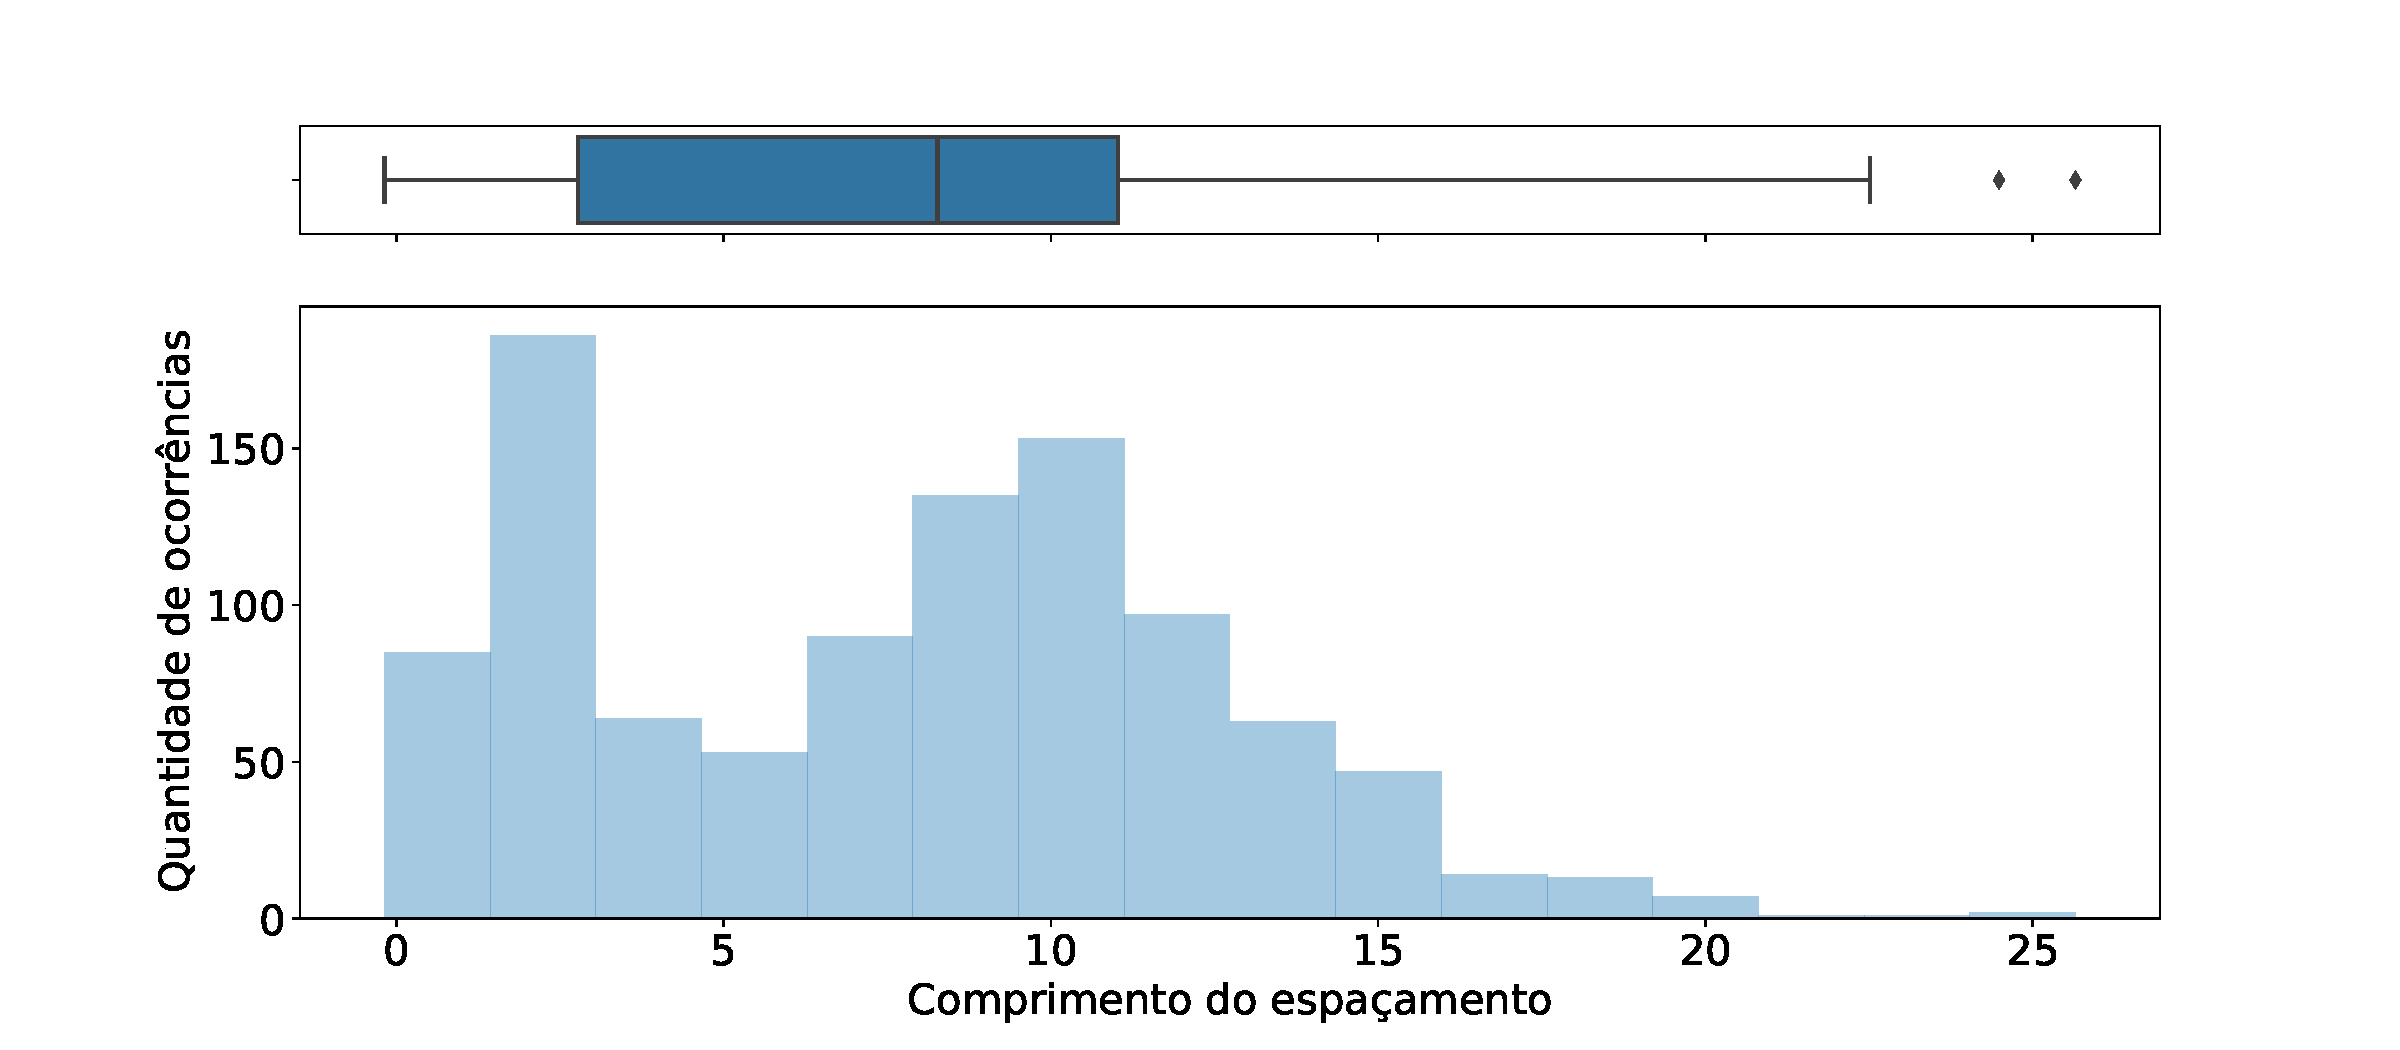
\includegraphics[width=\linewidth]{images/figuras/Espaçamento médio entre as colunas.pdf} }}%
    \hfill
    
    \subfloat[\centering Espaçamento entre as colunas para cada categoria de busca ]{{\includegraphics[width=\linewidth]{images/figuras/Espaçamento entre colunas por cada categoria de busca.pdf} }}%

    \hfill
   

    \caption{Análise do espaçamento entre as colunas}
    \label{fig:spac_colunas}
\end{figure}


Em resumo, o que estes dados nos sugerem é que a construção de um procedimento que linearize os documentos é uma tarefa possível, já que algum tipo de comportamento padrão foi observado. 






\section {Análise de contexto}

% Apesar dos formatos variados, decidimos aplicar ferramentas básicas de processamento de linguagem natural para obter melhores insights sobre os textos. 

% Primeiramente, carregamos os textos como observações em uma "data.frame" do módulo pandas. 

% Usando o módulo \textit{nltk}, experimentamos a função \textit{concordance} para identificar o contexto de termos de interesse no corpus. Contudo, essa função requer um processo de tokenização e, na implementação do \textit{word tokenize} do módulo \textit{ntlk}, os espaços são removidos. Isso não é interessante para a fazer análise exploratória, pois a presença de espaços repetidos indicam a segmentação do documento em colunas. 

% Com base no resultado da função menciona acima, resolvemos criar uma função parecida para o nosso contexto e que capture o entorno, mantendo os espaços repetidos. 




\subsection{Avaliando o entorno dos termos buscados}


Nesta seção iremos avaliar o contexto dos termos de busca através de uma inspeção das palavras do entorno do termo utilizado para busca.
Apesar dos formatos variados, decidimos aplicar ferramentas básicas de processamento de linguagem natural para obter melhores \textit{insights} sobre os textos. 

Para realizar tal tarefa, inicialmente utilizamos a ferramenta \textit{NLTK}, que é uma biblioteca em Python para utilização em atividades de processamento de linguagem natural. Com ela podemos transformar o texto em conjuntos de \textit{Tokens}. Um \textit{Token} é o nome técnico para um sequência de caracteres que queremos tratar como uma unidade, tais como "cabelo" e "violão". 
Uma ferramenta que nos interessa para esse momento é o "concordance". O "concordance" nos permite analisar os \textit{tokens} do entorno do termo de interesse. 


\begin{figure}[H]
    \centering
    \hfill
    
    \subfloat[\centering Análise de contexto baseado em \textit{tokens} do entorno. ]{{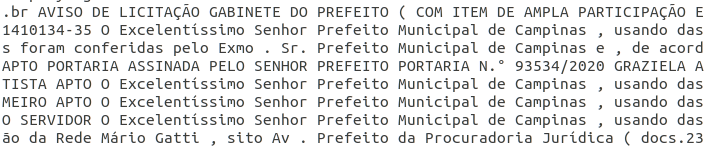
\includegraphics[width=0.8\linewidth]{images/prints/concordance_prefeito1.png} }}%
    \hfill
   
   \subfloat[\centering Análise de contexto baseado em caracteres do entorno. ]{{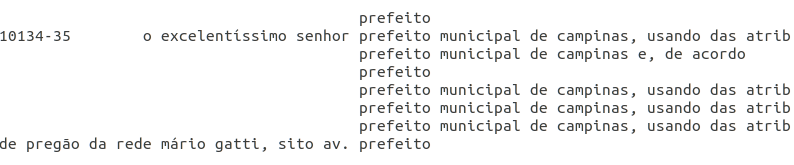
\includegraphics[width=0.8\linewidth]{images/prints/concordance_prefeito2.png} }}%
    \hfill
   
    \caption{Análise do contexto do termo "prefeito"}
    \label{fig:termo_prefeito}
\end{figure}

Na figura  \ref{fig:termo_prefeito}a temos a analise do termo "prefeito" utilizando o \textit{NLTK}. O resultado não nos serve para o momento pois a função não captura o problema do formato do arquivo com o qual estamos trabalhando (txt - linha continua) como comentado na seção anterior, além disso, a função não retorna informação para que possamos acumular o resultado em diferentes arquivos para uma análise mais extensiva, apenas a imprime no terminal.

Sendo assim, criamos uma função para análise de entorno do termo de interesse considerando uma quantidade fixa de caracteres antes e após o termo de interesse. Na figura \ref{fig:termo_prefeito}b temos um exemplo do resultado de avaliação do mesmo termo de busca no entanto com uma amostra de quantidade fixa de caracteres que o antecedem e o sucedem.

Utilizando a análise do entorno com base na quantidade de caracteres podemos verificar na figura \ref{fig:termo_teste_rapido} a importância da análise de colunas textuais presente nos documentos. Na primeira linha desta figura podemos perceber que a parte que antecede o termo de busca "teste rápido" se tratava de um texto colunar: ", apresentar a certidão de óbito; se divor-    " e após isso o termo buscado e as palavras que fazem sentido ao termo buscado "teste rápido coronavírus (covid19) ...".


\begin{figure}[H]
    \centering
    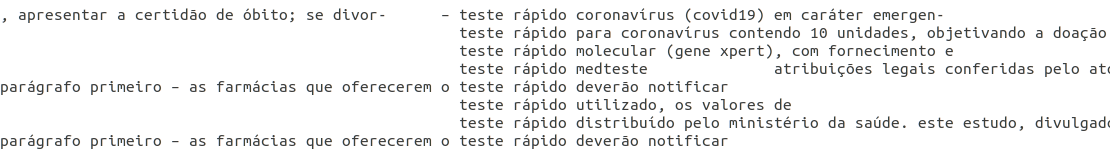
\includegraphics[width=\linewidth]{images/prints/concordance_teste_rapido.png}
        % Análise de contexto baseado em tokens do entorno.
    \caption{Análise do contexto do termo "prefeito"}
    \label{fig:termo_teste_rapido}
\end{figure}

Esta avaliação poderá nos auxiliar na busca de diferentes contextos para um termo de busca, identificar padrões que possam nos auxiliar nas implementações e como comentado, a importância da transformação de textos que se apresentam em colunas para um formato sequencial.

\subsection{Análise de palavras}

Após a \textit{tokenização}, para separar as sentenças em palavras que podemos obter uma informação que facilite o processamento e seu entendimento, dois filtros foram feitos, o primeiro retirando as \textit{stopwords}. \textit{Stopwords} são palavras comuns que pouco contribuem para o significado de uma frase. O \textit{NLTK} fornece um lista de \textit{stopwords} na língua portuguesa. 

Além disso, também incluímos algumas palavras específicas do contexto ao qual os diários oficiais são escrito. Após isso, retiramos palavras que tem menos de 4 caracteres, visto que após uma observação, percebemos que estas palavras, na maioria dos casos, eram pedaços de outras palavras resultante da quebra de linhas do texto.

Criamos um gráfico de barras que mostra as 30 palavras mais frequentes de todos os textos após serem filtrados os termos que não nos interessava.

% Gráfico de barras Frequência de palavras

\begin{figure}[H]
    \centering
    \includegraphics[scale=0.4]{images/figuras/freqência de palavras.pdf}
    \caption{Frequência de palavras}
    \label{fig:freq_palavras}
\end{figure}


As palavras apresentadas no gráfico \ref{fig:freq_palavras} aparecem muitas vezes nos nossos textos. Acreditamos que algumas delas possuem bastante relevância na extração de informações dos diários e que possam auxiliar na exploração e compreensão das medidas adotadas por municípios para enfrentar a pandemia do novo coronavírus.


\section{Conclusão}

% O objetivo deste trabalho foi entender o processo desde a origem dos dados que iremos trabalhar, nos poderes públicos, passando pela coleta feita pelos membros da OKF, no agrupamento por palavras-chave terminando no tipo de problema que eles querem uma solução. Percebemos que para a implementação de um
% \textit{framework} de cruzamento de levantamento de dados contra a corrupção, precisávamos entender mais a fundo o que de fato tínhamos à mão. Para isso, tomamos uma abordagem do dado concreto para uma informação abstrata: a linguagem.

% Verificar como os documentos estão dispostos em diretórios e qual o tamanho de cada um, assim como a presença de valores duplicados é essencial para verificar a viabilidade de processamento. Após esta etapa, iniciamos o processo de analisar o conteúdo dos arquivos, vendo como o texto estava formatado. Percebemos é bastante comum a presença de texto em múltiplas colunas além da presença de dados em tabelas, sem nenhum tipo de padrão aparente. Ao contar a quantidade de colunas por página, vimos que existe alguma padronização e que, por isso, seria possível executar algum procedimento que separe esse texto caso for necessário. Por último, uma análise semântica se viu necessário para que entendêssemos o contexto que cada documento estava inserido. Quais os jargões são os mais usados assim como quais informações apareciam nas redondezas das palavras-chave que foram utilizadas para a categorização dos arquivos.

% Durante o desenvolvimento da análise estatística descritiva, entendemos que esse processo nos deu entendimentos o suficiente para saber o terreno que devemos construir o produto desejado pelo cliente. 

% -----


O objetivo deste trabalho foi entender o processo: desde a origem dos dados que iremos trabalhar; passando pela coleta feita pelos membros da OKF, no agrupamento por palavras-chave; terminando no tipo de problema que eles pretendem solucionar. Este trabalho foi importante para percebemos que para a implementação de um \textit{framework} de cruzamento e levantamento de dados contra a corrupção, precisávamos entender mais a fundo o que de fato tínhamos em mãos. Para isso, tomamos uma abordagem partindo do dado concreto culminando para uma informação abstrata: a linguagem em si.

Verificamos como os documentos estão dispostos em diretórios e qual o tamanho de cada um. Identificamos presença de arquivos duplicados nos dados. Isso é importante conhecer pois pode influenciar bastante o processamento. 
Após esta etapa, realizamos o processo de analisar o conteúdo dos arquivos, mais especificamente no que tange a formatação. Percebemos que é bastante comum a presença de texto em múltiplas colunas, e presença de dados em tabelas diversas, sem nenhum tipo de padrão obvio. 
Ao contar a quantidade de colunas por página, vimos que existe alguma padronização e que, por isso, e isso nos instiga a investigar se é possível executar algum procedimento que separe esse texto caso venha a ser necessário. Por último, realizamos uma análise semântica. Esta se fez necessária para que pudéssemos entender o contexto que cada documento esta inserido. Isso nos permite, por exemplo, conhecer quais jargões são utilizados. Outra análise realizada foi a sobre as palavras que ocorriam nas redondezas das palavras-chave que foram utilizadas para a obtenção dos arquivos.

% to querendo concluir isso mas sei lá, não to curtindo mt do resultado

\end{document}